\section{Methodology}
The first step to performing successful data science experiments is obtaining good data. Therefore, this section first describes where data was obtained, how it was organized, and what precautions were practiced to avoid potential problems. Next the tools used are introduced along with the procedures and experiments performed.
\subsection{Data Collection}
For this study, all data was gathered from one institution, Southern Adventist University. Because the driving questions concern a typical classroom setting, the data collected needed to reflect only this setting.

Some courses at SAU only contained a handful of students per a semester. Additionally, several classrooms had movable desks. Because stickers on these desks indicated the seat row and column (as shown in Figure~\ref{fig:hsc1307}), adjustable desks could have introduced systematically flawed data in a study where seat placement is critical. To eliminate both of these issues, only physically large classrooms with bolted desks were selected.

Some faculty raised further concerns that the attendance system had changed as the university relaxed its COVID-19 restrictions. For instance, during its first semester of use, the attendance tracking system (ATS) only permitted students to sit in every other seat, thus restricting student seat choice. However, in following semesters, ATS allowed students to sit in any seat in a classroom. In favor of consistency, only the latter of these systems was used, resulting in two semesters of data (Fall 2021 and Winter 2022).

\begin{figure}[ht]
  \centering
  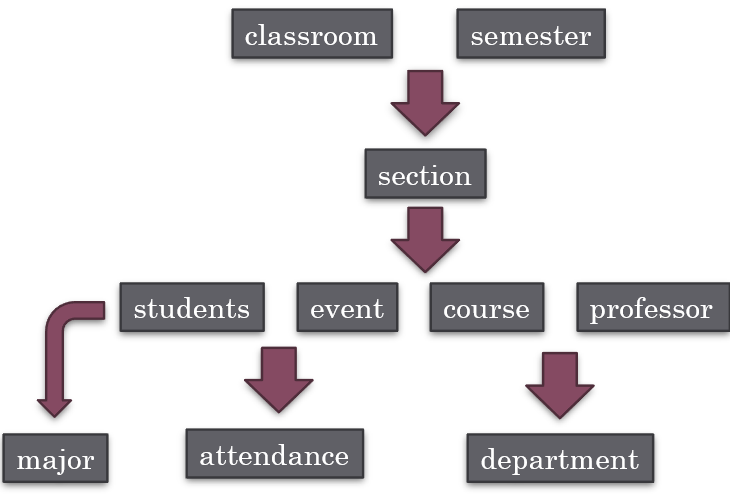
\includegraphics[width=0.48\textwidth]{figures/dataCollectionEntityTraversal.png}
  \caption{The natural progression of entities in data collection.}
  \label{fig:dataCollectionTraversal}
\end{figure}

Once locations and times were chosen for data collection, all other entities followed naturally as shown in Figure~\ref{fig:dataCollectionTraversal}. 159 course sections with twenty or more students enrolled were found using the seventeen chosen classrooms over the two semesters. 2,067 students were enrolled in one or more of these sections (see Figure~\ref{fig:demographics} for demographics) which were taught by sixty-three professors representing thirteen departments.

\begin{figure*}[ht]
  \centering
  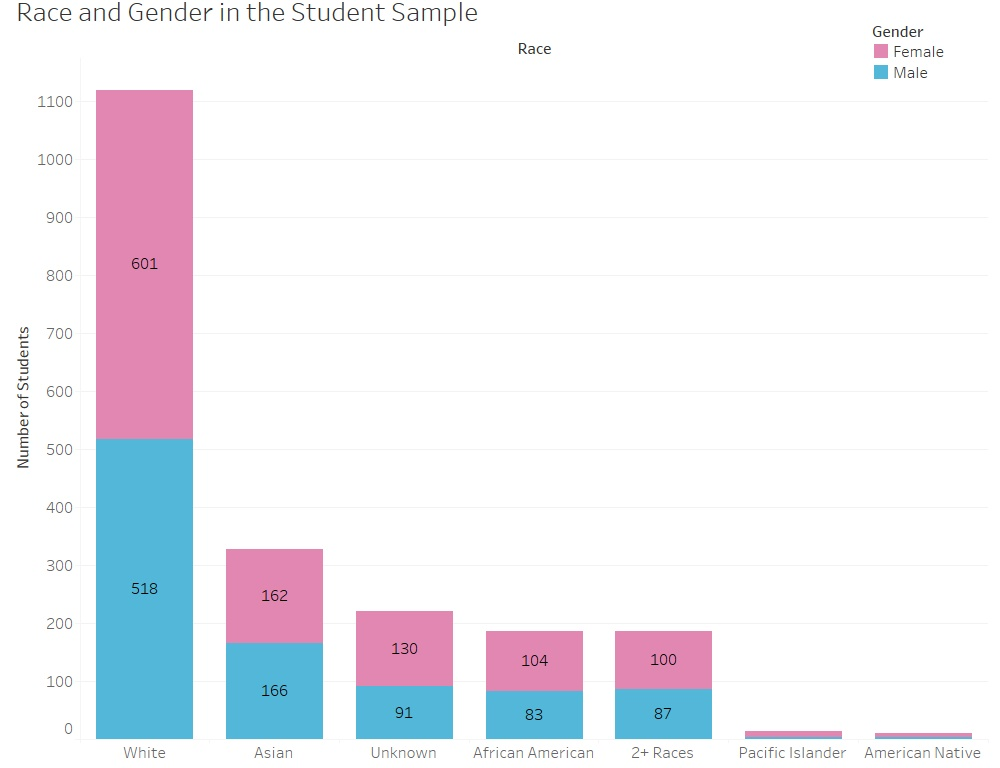
\includegraphics[width=\textwidth]{figures/demographics.jpg}
  \caption{Demographics of the students in our data. Graph created in Tableau.}
  \label{fig:demographics}
\end{figure*}

Each section had associated events that represented one class period. The ATS stored data for each student that was present, but it did not always specify if a student was absent from a class. Thus, using several structured query language (SQL) scripts, this data was imputed. If a student was enrolled in a section but had no record of attending any one of its events, they were assumed absent.

\subsection{Data Organization and Tools}
Dividing classes, students, and attendance into separate relations was the most natural way of storing and organizing the data. Because the data was pulled from a data warehouse partially external to the university, it was not separated this way. Thus, Tableau Prep Builder was used to segregate and clean the data.\footnote{\href{https://www.tableau.com/products/prep}{tableau.com/products/prep}}

Because Microsoft Azure was to be used for the data science experiments, it was also chosen to store and serve the data. Using an Azure SQL Database on an Azure SQL Server, we constructed a relational database from the outputs of Tableau Prep Builder. After resolving all the bugs encountered during data collection, the cleaned CSV files provided by Tableau Prep Builder were simply imported as tables into the database using Microsoft SQL Server Management Studio (SSMS). Primary and foreign keys were also configured in SSMS. The resulting schema for this database can be seen in Figure~\ref{fig:schema}. All entities are transitively related using primary/foreign keys.

\begin{figure}[ht]
  \centering
  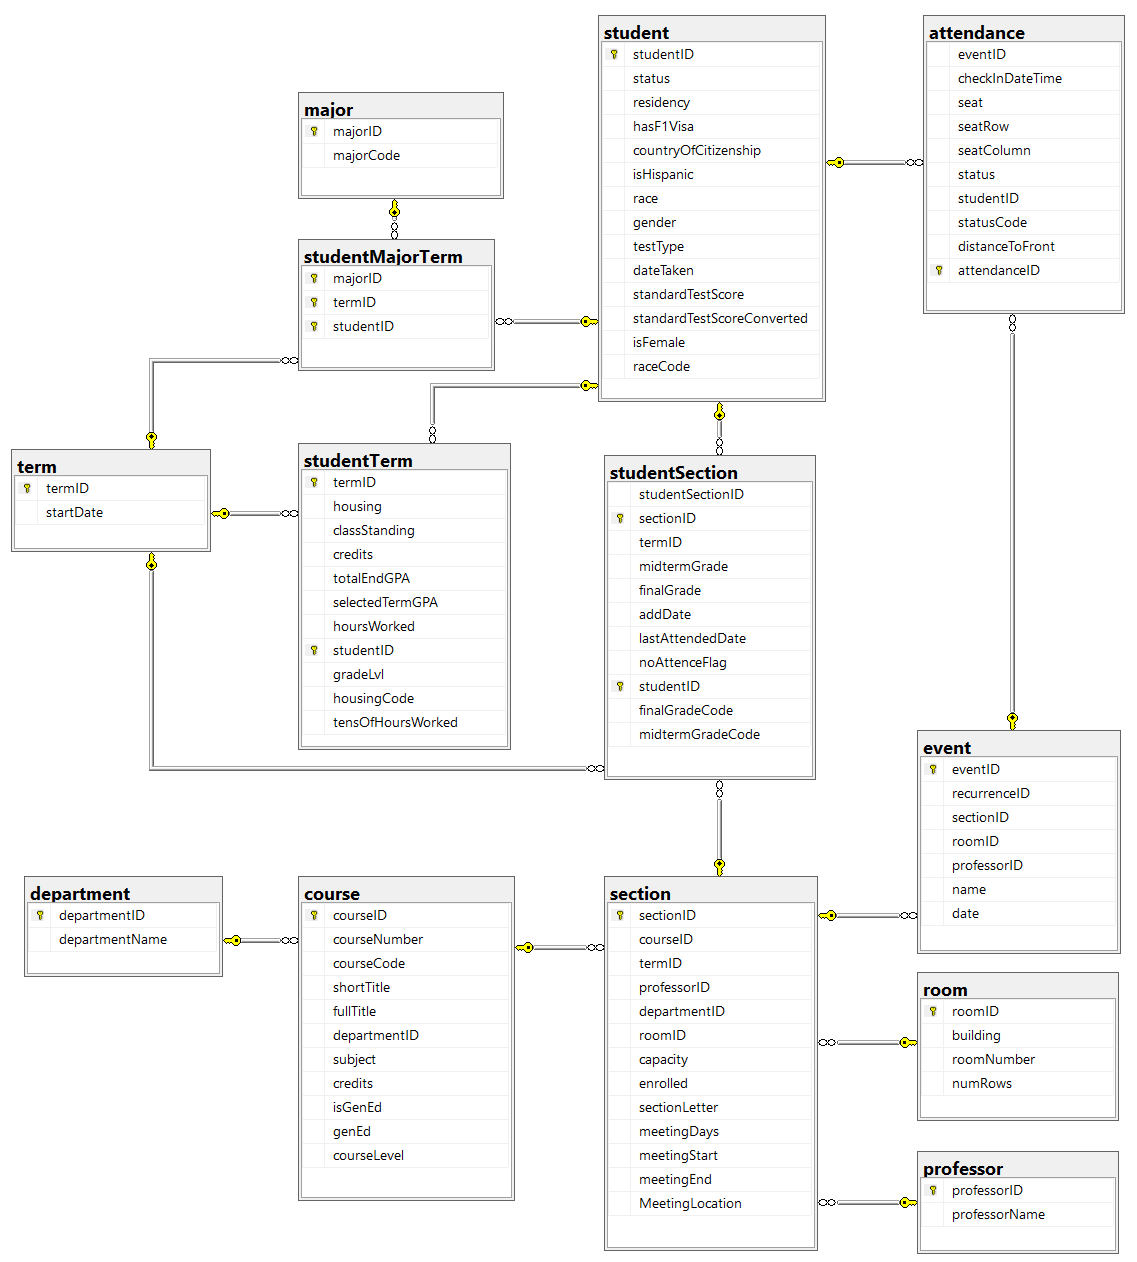
\includegraphics[width=0.48\textwidth]{figures/attendanceDBSchema.png}
  \caption{An abbreviated form of the database schema as visualized by Microsoft SQL Server Management Studio.}
  \label{fig:schema}
\end{figure}

The initial reasons for using Microsoft Azure were its advertized ease of use and Automated Machine Learning workspace (AutoML). AutoML is an emerging technology that offers automatic training of various machine learning models without the need for code.

In a typical solution, data is first supplied to a model training component. The component trains a prediction model, often even automatically choosing which algorithm is best for solving a given classification, regression, clustering, or forecasting problem. It may also tune the model's hyperparameters.

\subsection{Experiment Plan}
The general plan for regression and clustering experiments was to connect the Azure AutoML workspace to the Azure SQL Database so that the AutoML components could automatically extract the latest data from the database. Using these two platforms, we created automatic pipelines that built machine learning models for student grades. Finally, various subsets of attributes were provided to the AutoML pipeline to run experiments on.

After producing a model, Azure supplied various metrics associated with that model. For regression, these included error scores and correlation coefficients, allowing for a simple correlation analysis of any subset of attributes. For clustering models, metrics included cluster densities and diameters as well as each record's cluster assignment. Using this information, the model could provide the average values of each attribute in each cluster, which could give insight into how the algorithm naturally organized the data.

To perform logistic regression and data clustering, class data first needed to be transformed into a numerical format. The twelve grade categories ``A-F'' were converted to the numbers 1-12, respectively. Also, ``I'' (incomplete) and ``IP'' (incomplete passing) were assigned values of 13 and 14.\footnote{This assumes that not completing a class is a less favorable outcome than failing it. Also ``Incomplete Passing'' is marked as lower than ``Incomplete,'' but it is not a cause for concern as this represents less than 0.1\% of the data.}

Other categorical variables were converted in a similar manner. For example, there were five categories for attendance status. The labels ``Present,'' ``Online,'' ``Late,'' ``Excused,'' and ``Absent'' were assigned the values 0-4 respectively.

Further, as shown in the ATS interface in Figure~\ref{fig:hsc1307}, students selected their seat using a numerical column and a {\it row letter}. Most training models would perform better with a {\it row number} rather than a letter. Also, the number of rows and spacing between those rows in each classroom varied, rendering any categorical row data inconsistent. To provide the most useful data to the algorithms that would train our models, the row letters were extracted, aggregated for each classroom, and converted to a normalized distance from the front of the classroom. This new attribute, called ``distanceToFront,'' measured how far a student's chosen seat was from the front of the classroom. Values closer to ``$0$'' indicate seats closer to the front row of a classroom while those closer to ``$1$'' represent seats at the back of a classroom.

The final query fetches the attributes of interest for this project (shown below).\footnote{Notice that courses in the Nursing (NRSG) and Physical Education (PEAC) departments were filtered out. Nursing courses were removed because students were often assigned seats in these courses, thus removing the student's ability to choose their seat. Physical education courses, on the other hand, were not considered a "normal classroom setting."} These attributes included student demographic information, credit load, hours worked during the semester, distance to the front of the classroom, attendance status, and final grade. This query was run against the Azure SQL database and the resulting data was used as a starting point for Azure's AutoML experiments.
\begin{lstlisting}[language=SQL]
select s.isFemale, s.isHispanic, s.race,
	st.housing, st.gradeLevel, st.credits, 
  st.tensOfHoursWorked,
	a.distanceToFront, a.seatColumn, a.statusCode,
	sn.finalGradeCode
from attendance a
	join student s on a.studentID = s.studentID 
	join studentTerm st on s.studentID = st.studentID
	join studentSection sn on s.studentID = sn.studentID 
    and sn.termID = st.termID
	join section n on sn.sectionID = n.sectionID
	join event e on n.sectionID = e.sectionID and e.eventID = a.eventID
	join course c on n.courseID = c.courseID
where c.departmentID != 'NRSG' 
  and c.departmentID != 'PEAC';
\end{lstlisting}

\subsubsection{Correlation Analysis}
Regression experiments were configured as ``jobs'' and started in Azure's Machine Learning Workspace. To analyze correlation across different groups of attributes, the experiment was run multiple times with different subsets of the columns shown in the query above. The experiments and their results are presented in the ``Results'' section.
\subsubsection{Clustering}
While regression can show correlation between sets of independent and dependent variables, it does not allow an algorithm to make its own conclusions about the data. However, clustering algorithms can take data and learn to organize it. This is a classic example of unsupervised learning. Rather than telling the algorithm how the data should be fit, unsupervised learning allows the model to try to group the data based on all the given attributes. After the algorithm has formed clusters of data that minimize some cost function, the clusters can be assessed to form conclusions.

Azure's AutoML platform can perform popular clustering algorithms such as K-means. Perfecting these experiments was the longest part of this project. However, after many cycles of trial, error, research, and reconfiguration, we arrived at an abstract, streamlined clustering solution.

\begin{figure*}[ht]
  \centering
  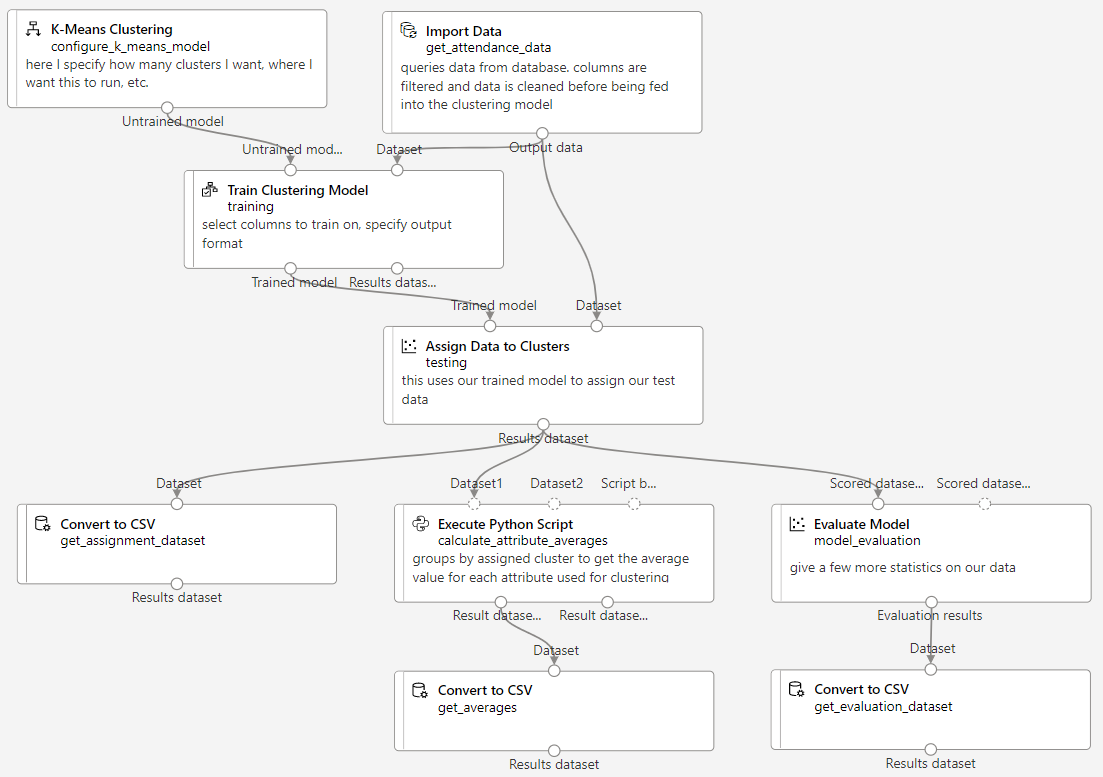
\includegraphics[width=\textwidth]{figures/clusteringPipeline.png}
  \caption{The clustering pipeline used in this project. Note that to make this image fit better on paper, a data cleaning step and a column selection step were removed from the pipeline. The cleaning step simply imputed missing values using column means.}
  \label{fig:clusteringPipeline}
\end{figure*}

This solution was created as a pipeline. In a pipeline, several components can be ``wired together'' to create a single process. This process is capable of gathering data, processing it, training machine learning models, testing those models, and generating result data in automatic succession. The machine learning pipeline shown in Figure~\ref{fig:clusteringPipeline} was used to perform clustering for this project.

In the {\bf Import Data} component (top right), the pipeline fetches data dynamically from the Azure SQL Database. Different attributes can be selected within or after the query that this component performs. Initially, numerical, textual, and categorical data was being returned. However, after several experiments and database adjustments, only numerical data was fetched using query shown above.

On the top left, the {\bf K-Means Clustering} component is used to initialize and configure an untrained clustering model. Several parameters can be set here: the number of clusters desired in the output, the feature normalization option, a model weight initialization algorithm, and a multi-dimensional distance metric.\footnote{In our experiments, the number of clusters varied from two to fourteen, normalization was enabled, weights were initialized with the ``K-Means++'' algorithm, and a Euclidean distance metric was used.} The {\bf Train Clustering Model} component then trains this model using the imported data.

  {\bf Assign Data to Clusters} takes all the provided data and assigns it to a cluster using the trained model. Using this data, the model can be evaluated in the {\bf Evaluate Model} block which measures average distances between all clusters. It may be possible to generate more evaluation metrics, but we were not able to achieve these results because documentation for this component was inconsistent and generally lacking.

Luckily, Azure provides a mechanism for executing Python code anywhere\footnote{anywhere that the proper input and outputs can be wired, that is} in a pipeline. A custom Python script only needs to contain an \lstinline{azureml_main()} function that receives and returns up to two dataframes.\footnote{A dataframe is just a specific format for a table of data usually managed by the \lstinline{pandas} library.} The rest is up to the pipeline designer. To generate the necessary data, {\bf Execute Python Script} receives all the records along with their cluster assignments and calculates the average value of every feature for each cluster (see code below).
\begin{lstlisting}[language=Python]
  import pandas as pd
  def azureml_main(dataset, optional_data = None):
      return dataset.groupby("Assignments").mean()
\end{lstlisting}

Finally, all the data generated by these components is converted into comma-separated value (CSV) format. The results are discussed below.

